% Options for packages loaded elsewhere
\PassOptionsToPackage{unicode}{hyperref}
\PassOptionsToPackage{hyphens}{url}
%
\documentclass[
]{article}
\usepackage{amsmath,amssymb}
\usepackage{lmodern}
\usepackage{iftex}
\ifPDFTeX
  \usepackage[T1]{fontenc}
  \usepackage[utf8]{inputenc}
  \usepackage{textcomp} % provide euro and other symbols
\else % if luatex or xetex
  \usepackage{unicode-math}
  \defaultfontfeatures{Scale=MatchLowercase}
  \defaultfontfeatures[\rmfamily]{Ligatures=TeX,Scale=1}
\fi
% Use upquote if available, for straight quotes in verbatim environments
\IfFileExists{upquote.sty}{\usepackage{upquote}}{}
\IfFileExists{microtype.sty}{% use microtype if available
  \usepackage[]{microtype}
  \UseMicrotypeSet[protrusion]{basicmath} % disable protrusion for tt fonts
}{}
\makeatletter
\@ifundefined{KOMAClassName}{% if non-KOMA class
  \IfFileExists{parskip.sty}{%
    \usepackage{parskip}
  }{% else
    \setlength{\parindent}{0pt}
    \setlength{\parskip}{6pt plus 2pt minus 1pt}}
}{% if KOMA class
  \KOMAoptions{parskip=half}}
\makeatother
\usepackage{xcolor}
\usepackage{graphicx}
\makeatletter
\def\maxwidth{\ifdim\Gin@nat@width>\linewidth\linewidth\else\Gin@nat@width\fi}
\def\maxheight{\ifdim\Gin@nat@height>\textheight\textheight\else\Gin@nat@height\fi}
\makeatother
% Scale images if necessary, so that they will not overflow the page
% margins by default, and it is still possible to overwrite the defaults
% using explicit options in \includegraphics[width, height, ...]{}
\setkeys{Gin}{width=\maxwidth,height=\maxheight,keepaspectratio}
% Set default figure placement to htbp
\makeatletter
\def\fps@figure{htbp}
\makeatother
\setlength{\emergencystretch}{3em} % prevent overfull lines
\providecommand{\tightlist}{%
  \setlength{\itemsep}{0pt}\setlength{\parskip}{0pt}}
\setcounter{secnumdepth}{-\maxdimen} % remove section numbering
\ifLuaTeX
  \usepackage{selnolig}  % disable illegal ligatures
\fi
\IfFileExists{bookmark.sty}{\usepackage{bookmark}}{\usepackage{hyperref}}
\IfFileExists{xurl.sty}{\usepackage{xurl}}{} % add URL line breaks if available
\urlstyle{same} % disable monospaced font for URLs
\hypersetup{
  hidelinks,
  pdfcreator={LaTeX via pandoc}}

\author{}
\date{}

\begin{document}

\begin{center}
\textbf{FITNESS LANDSCAPE ANALYSIS FOR HILL CLIMBING ALGORITHMS}
\end{center}

Author: Negura Teodor Alexandru

\begin{center}
\textbf{ABSTRACT}
\end{center}

This report analyzes how two Hill Climbing variants perceive and
navigate the same optimization landscape. We study a cubic function over
a discrete domain with thirty-two possible solutions. Best Improvement
evaluates all neighbors before moving, achieving eighty-seven percent
success in finding the global optimum. First Improvement moves to the
first better neighbor found, achieving only forty-four percent success.
The results demonstrate that algorithmic strategy fundamentally shapes
landscape difficulty: the same problem appears easy to one algorithm and
hard to another.

\begin{center}
\textbf{INTRODUCTION}
\end{center}

This study investigates the relationship between optimization algorithms
and fitness landscapes. We examine how different Hill Climbing
strategies navigate the same mathematical function, revealing that
problem difficulty emerges from the interaction between the landscape
and the algorithm, not just from the objective function itself. We
analyze a cubic polynomial function over a discrete domain of thirty-two
solutions. This small search space allows complete analysis while
providing clear insights into local search behavior.

\textbf{Motivation}

Understanding fitness landscapes matters because different landscapes
favor different optimization strategies. By analyzing how algorithms
perceive landscapes, we can predict performance and select appropriate
methods. This study provides concrete evidence for theoretical claims
about local search behavior, making abstract concepts tangible for
computer science students.

\textbf{Problem Description}

We maximize a cubic
function over integer values from zero to thirty-one. Each solution has
exactly five neighbors that differ by one position in their
representation. The problem has four local maxima: three are traps with
suboptimal values, and one is the global optimum we seek to find.

\begin{center}
\textbf{METHODS}
\end{center}

Hill Climbing iteratively moves from the current solution to a better
neighboring solution. The algorithm starts at some point, evaluates
neighbors, selects one to move to, and repeats until no improving
neighbor exists. At this point, it has reached a local maximum and
terminates. We use a discrete representation where each solution has
exactly five neighbors. To ensure comprehensive analysis, we test every
possible starting point rather than using random initialization. This
eliminates sampling bias and provides exact measurements of algorithm
behavior. The algorithm terminates when reaching a local maximum,
defined as a solution where all neighbors have equal or worse fitness.

\textbf{Algorithm Variants}

Best Improvement evaluates all five neighbors at each
step and selects the one with maximum fitness improvement. This
exhaustive strategy provides complete neighborhood information and
chooses the steepest ascent direction. It costs five evaluations per
iteration but makes informed decisions. First Improvement evaluates
neighbors in a fixed order and immediately moves to the first neighbor
that improves fitness. This eager strategy may evaluate as few as one
neighbor or as many as five. It saves computational cost but makes
myopic decisions without seeing all alternatives.

\begin{center}
\textbf{EXPERIMENTAL SETUP}
\end{center}

We test both algorithms from all thirty-two possible starting points.
This exhaustive approach provides complete characterization of algorithm
behavior without statistical uncertainty. Each run uses exact integer
arithmetic with no approximation errors.

\begin{center}
\textbf{STATIC LANDSCAPE ANALYSIS}
\end{center}

Through exhaustive evaluation, we identify exactly four local maxima in
the fitness landscape. The global optimum has fitness four thousand one
hundred. Three local traps exist with fitness values of three thousand
eight hundred three, three thousand nine hundred eighty-eight, and three
thousand two hundred thirty-six. These traps are peaks where all
neighbors have lower fitness, potentially capturing algorithms that
climb to them. Figure 1 shows the complete fitness landscape with all
local maxima marked.

\begin{center}
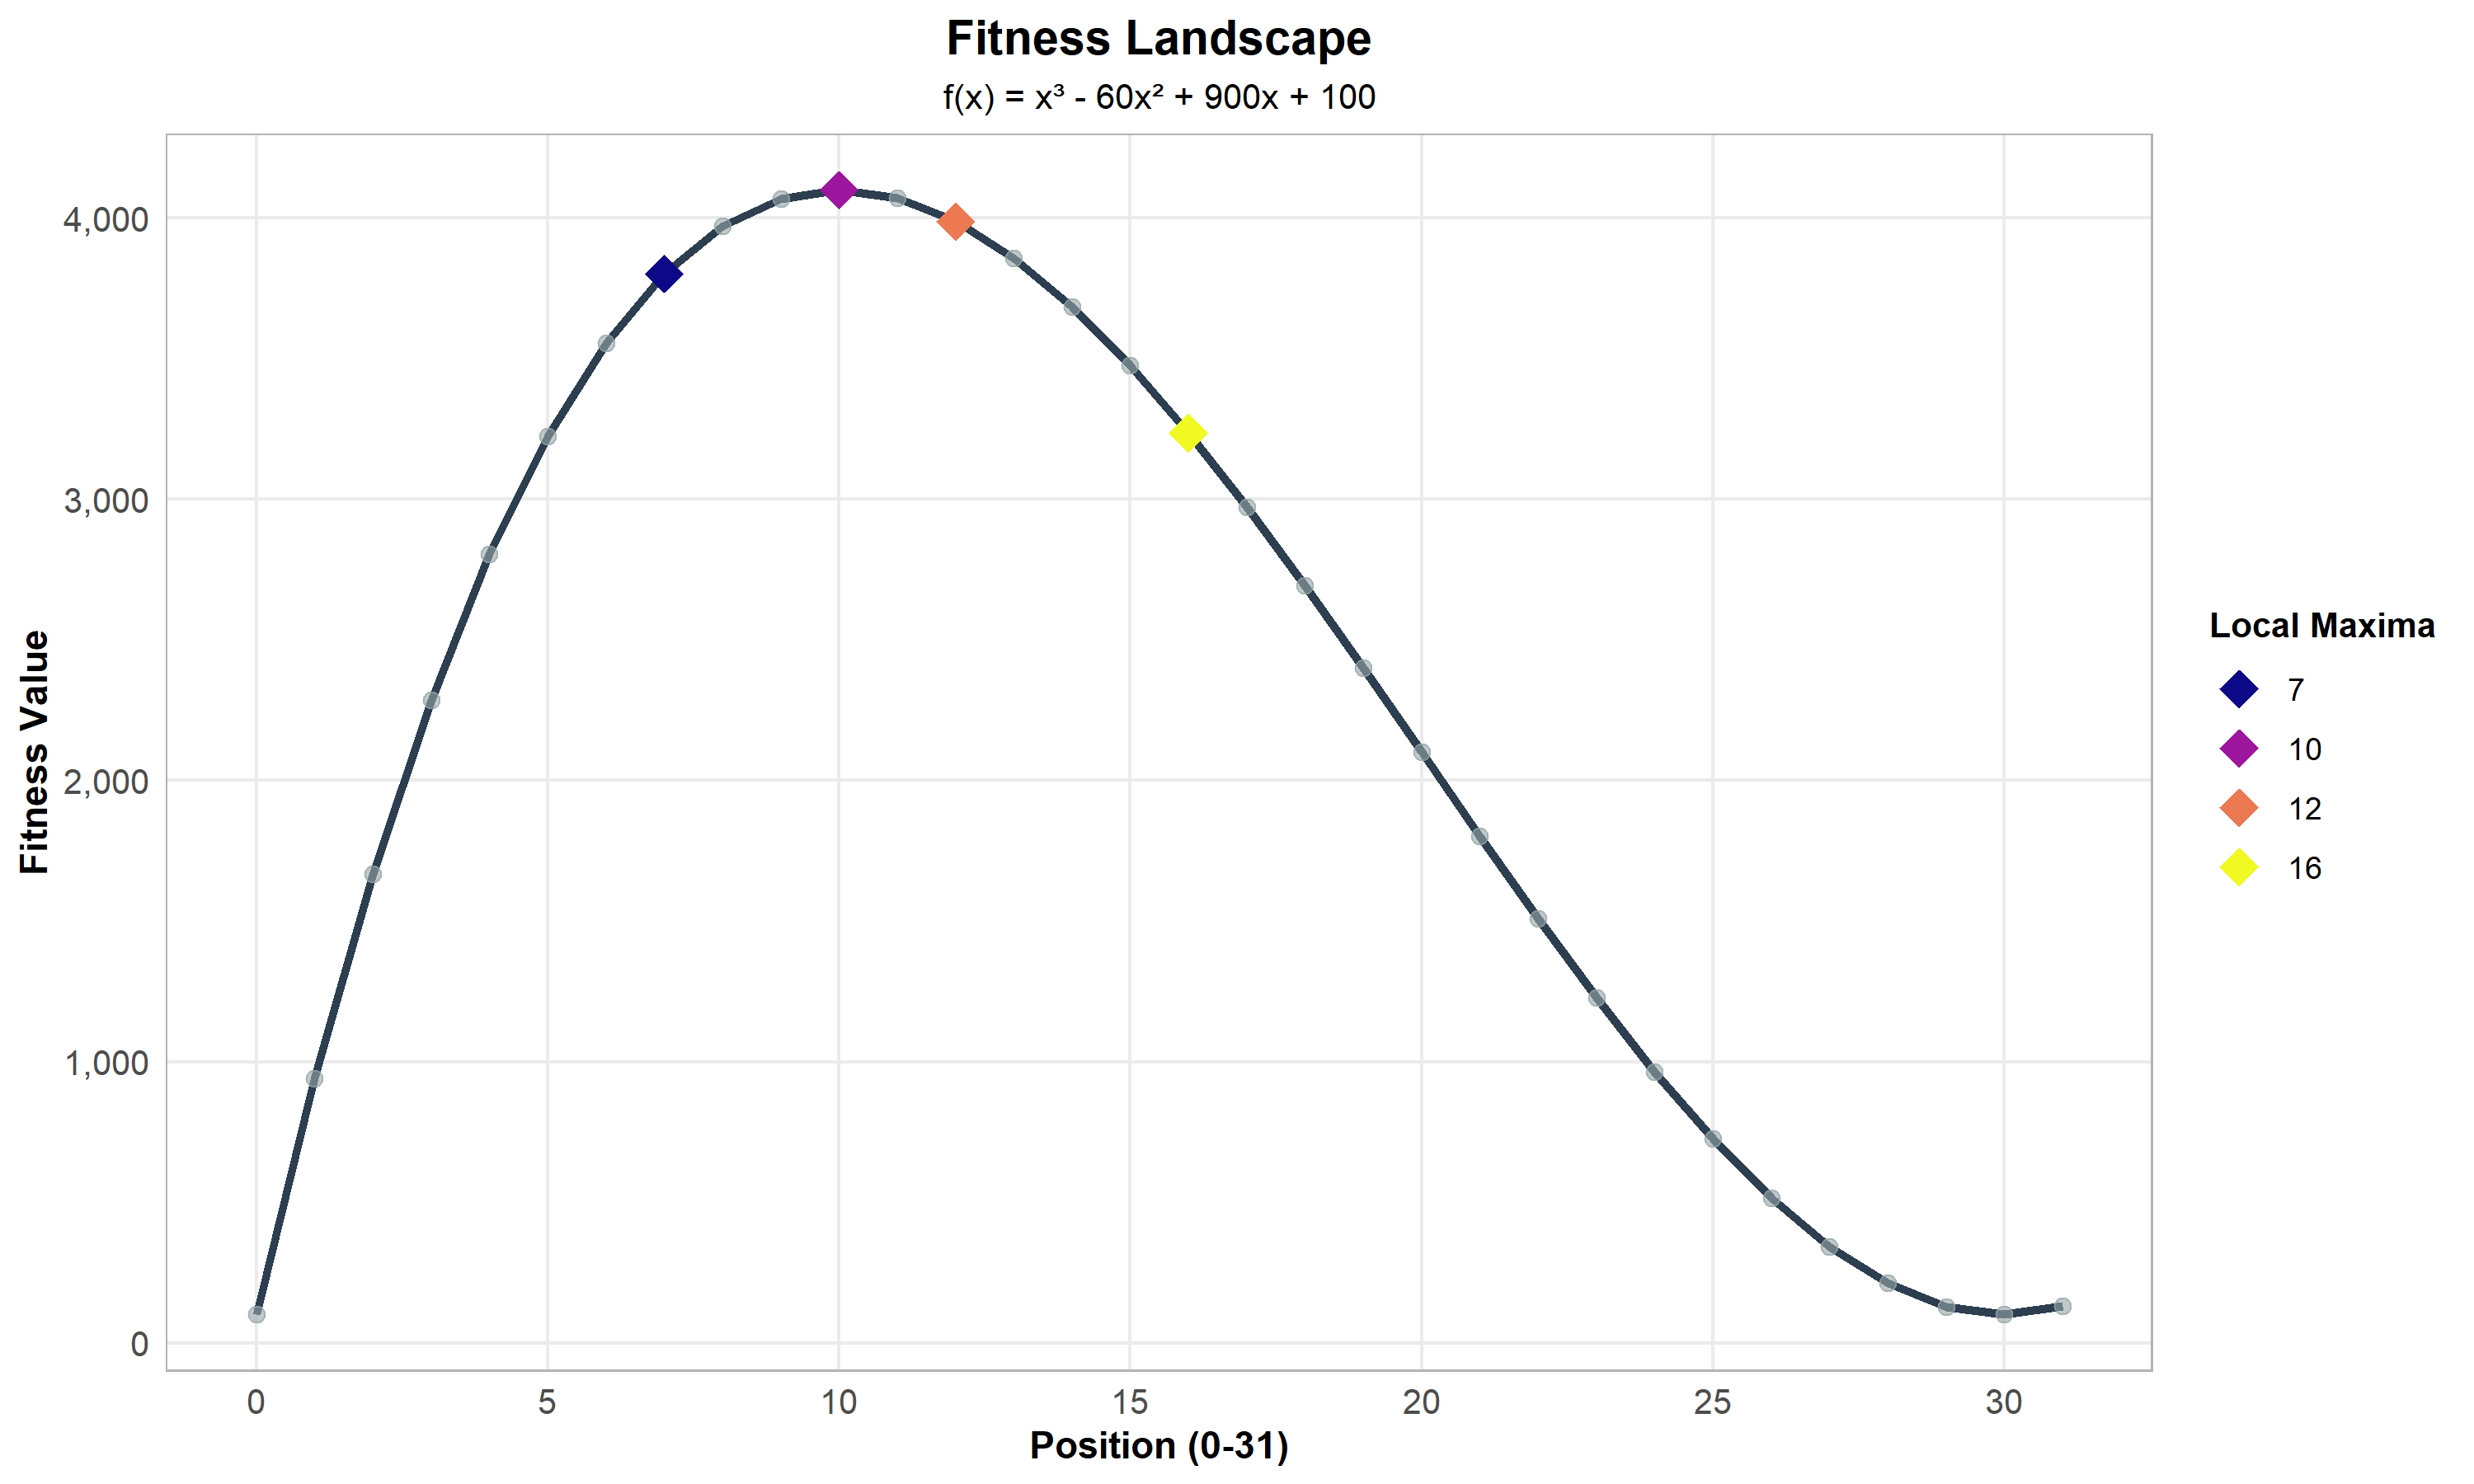
\includegraphics[width=5in]{../landscape_plot.png}
\par\textit{Figure 1: Fitness landscape showing all local maxima}
\end{center}

\begin{center}
\textbf{EXPERIMENTAL RESULTS}
\end{center}

Best Improvement demonstrates exceptional robustness. Twenty-eight out
of thirty-two starting points converge to the global optimum, achieving
eighty-seven percent success. Only four runs terminate at local traps.
The algorithm creates a simplified perception of the landscape where the
global optimum dominates with a vast attraction basin covering most of
the search space.

\textbf{First Improvement Performance}

First Improvement shows
high sensitivity to initialization. Only fourteen out of thirty-two
starting points reach the global optimum, achieving forty-four percent
success. Eleven runs trap at the first local maximum, four trap at the
second, and three trap at the third. The algorithm fragments the search
space into four competing basins of similar sizes. Figure 2 illustrates
how First Improvement makes point-to-point jumps, showing the myopic
nature of its decisions.

\begin{center}
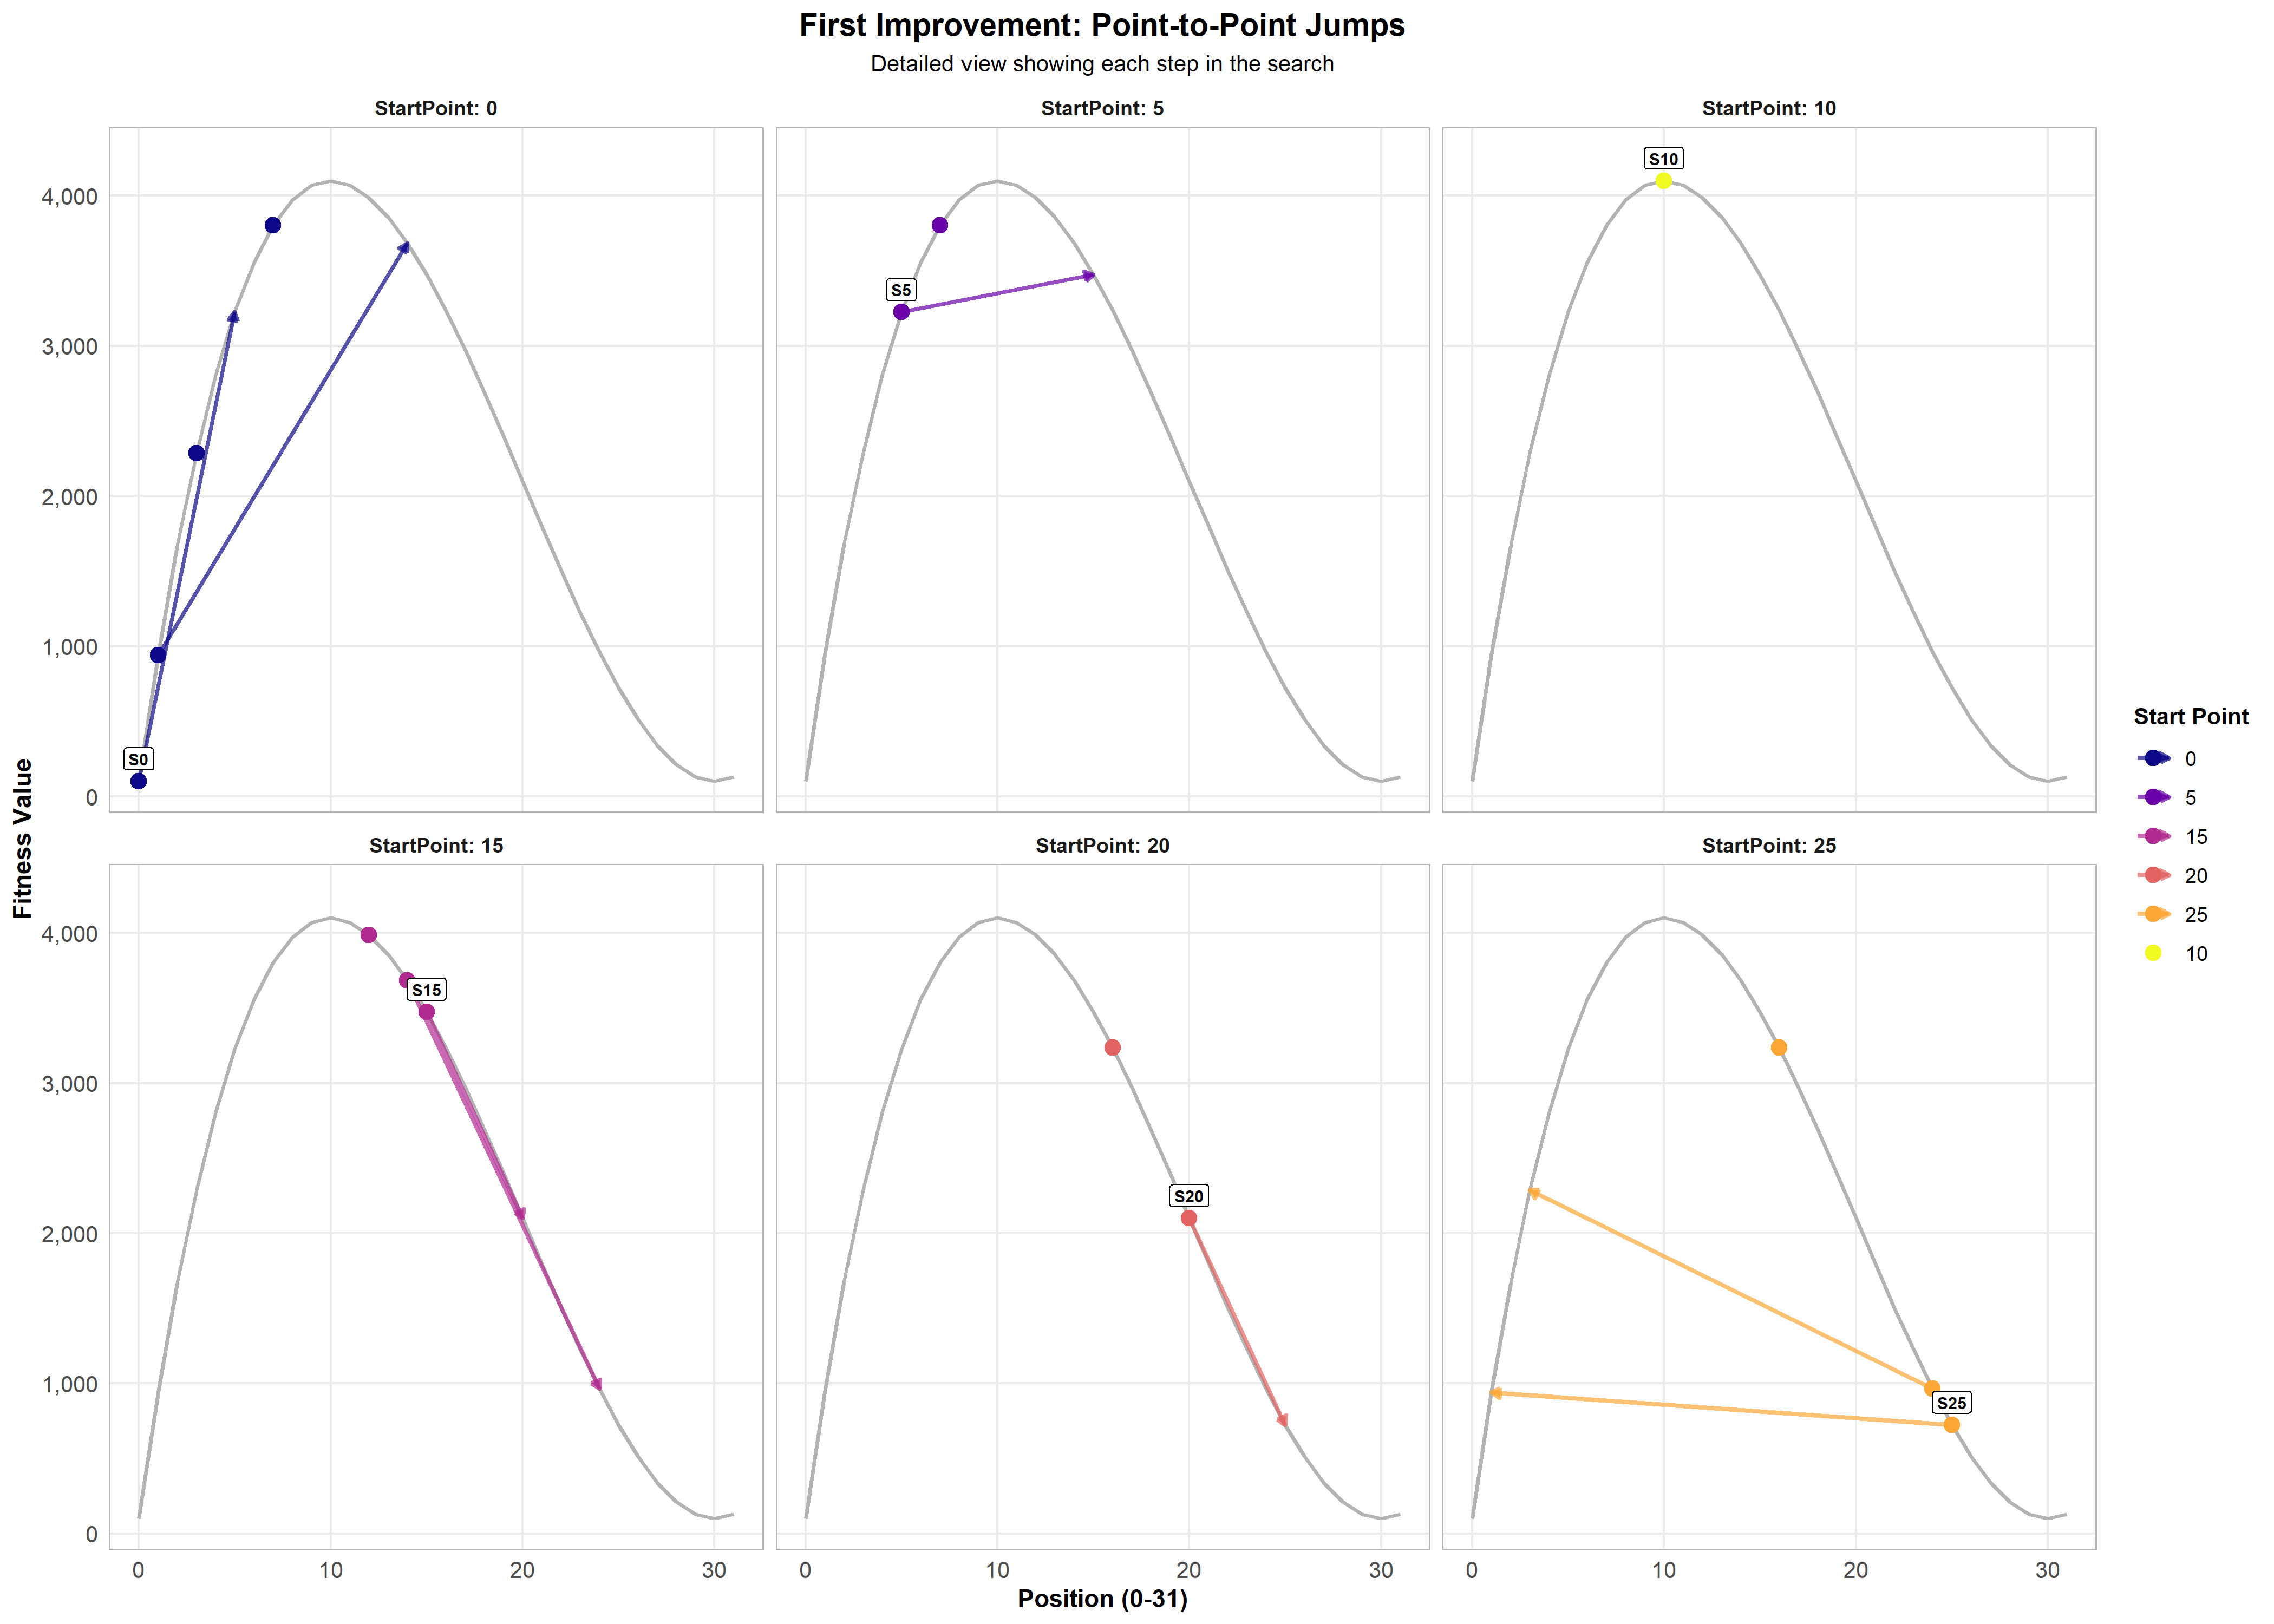
\includegraphics[width=6in]{../fi_detailed_jumps.png}
\par\textit{Figure 2: First Improvement trajectories showing step-by-step jumps from different starting points}
\end{center}

\textbf{Comparative Analysis}

Best Improvement achieves double the success rate of First Improvement.
While Best Improvement requires about one point eight times more
evaluations per iteration, this modest cost increase yields dramatically
improved solution quality. The same physical landscape appears smooth
and navigable to Best Improvement but rugged and treacherous
to First Improvement. Figure 3 directly compares both algorithms' paths
from identical starting points, revealing their different navigation strategies.

\begin{center}
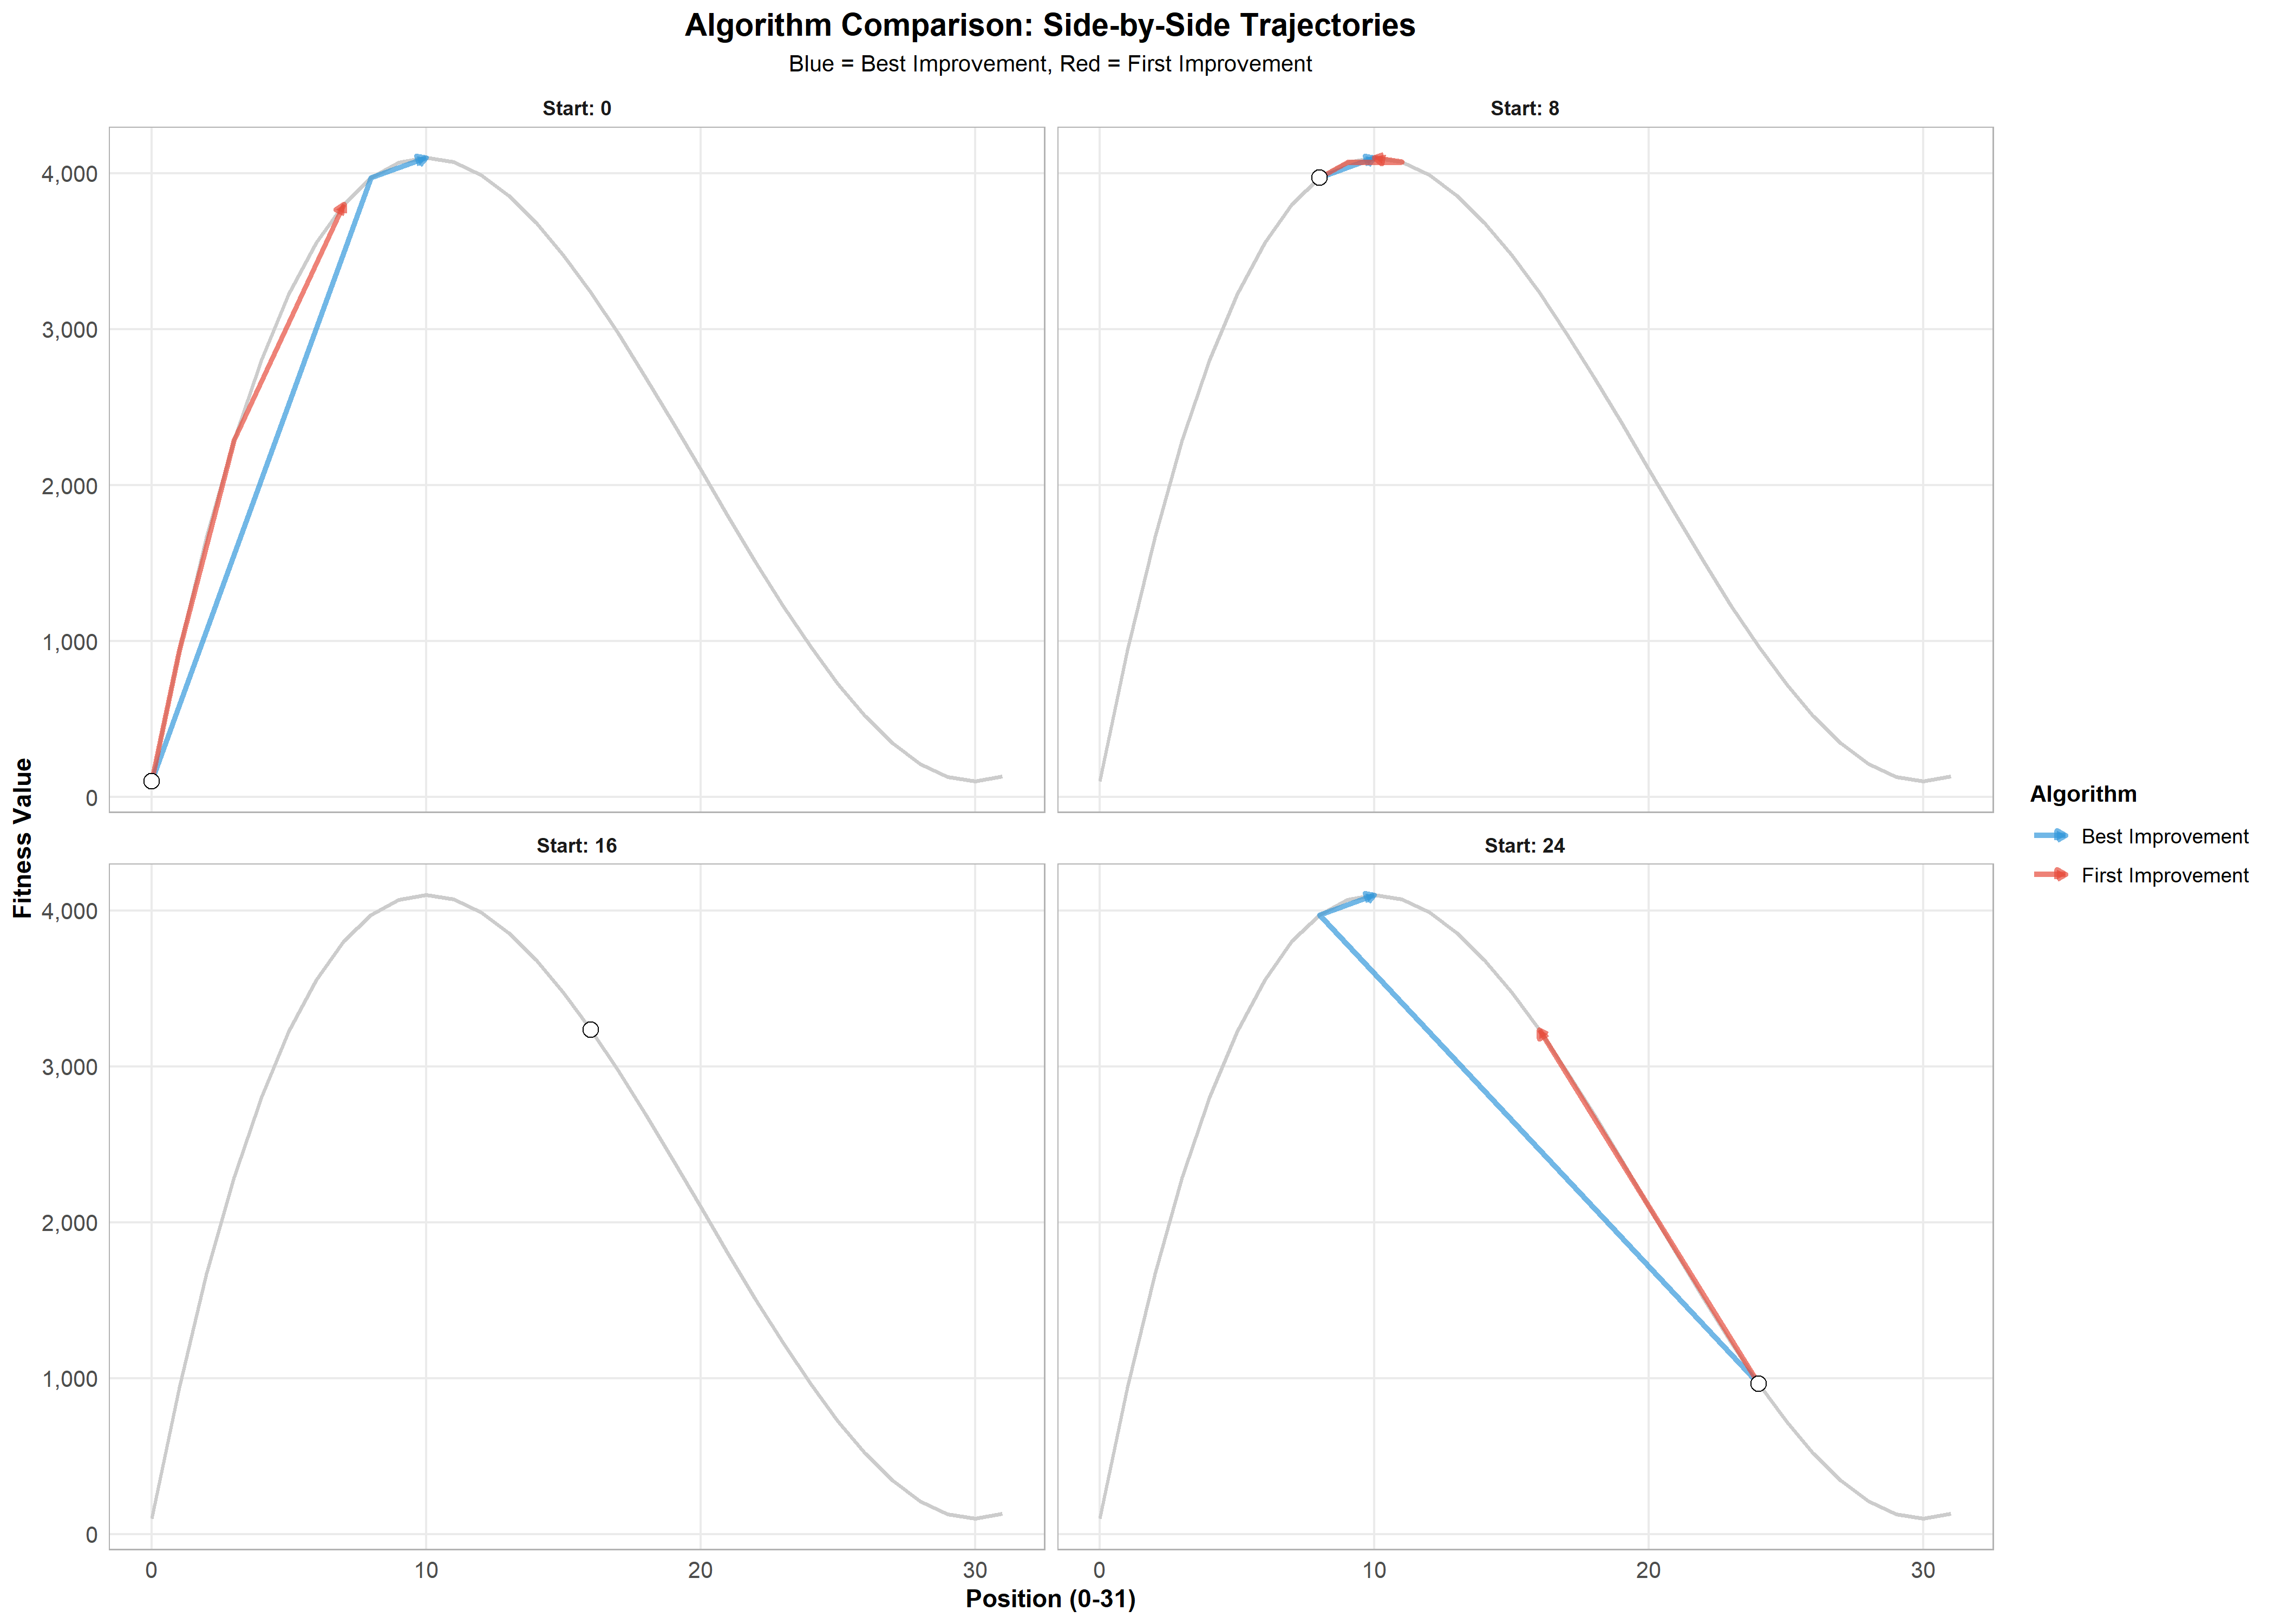
\includegraphics[width=6in]{../algorithm_comparison.png}
\par\textit{Figure 3: Side-by-side comparison of Best Improvement (blue) vs First Improvement (red) from the same starting points}
\end{center}

\begin{center}
\textbf{COMPARISON AND DISCUSSION}
\end{center}

When allowed one hundred evaluations maximum, Best Improvement produces
solutions averaging four thousand forty-seven in fitness, while First
Improvement averages three thousand eight hundred sixty-one. Even with
the same computational budget, Best Improvement delivers higher quality
solutions. Figure 4 quantifies the success rates and basin sizes for
both algorithms.

\begin{center}
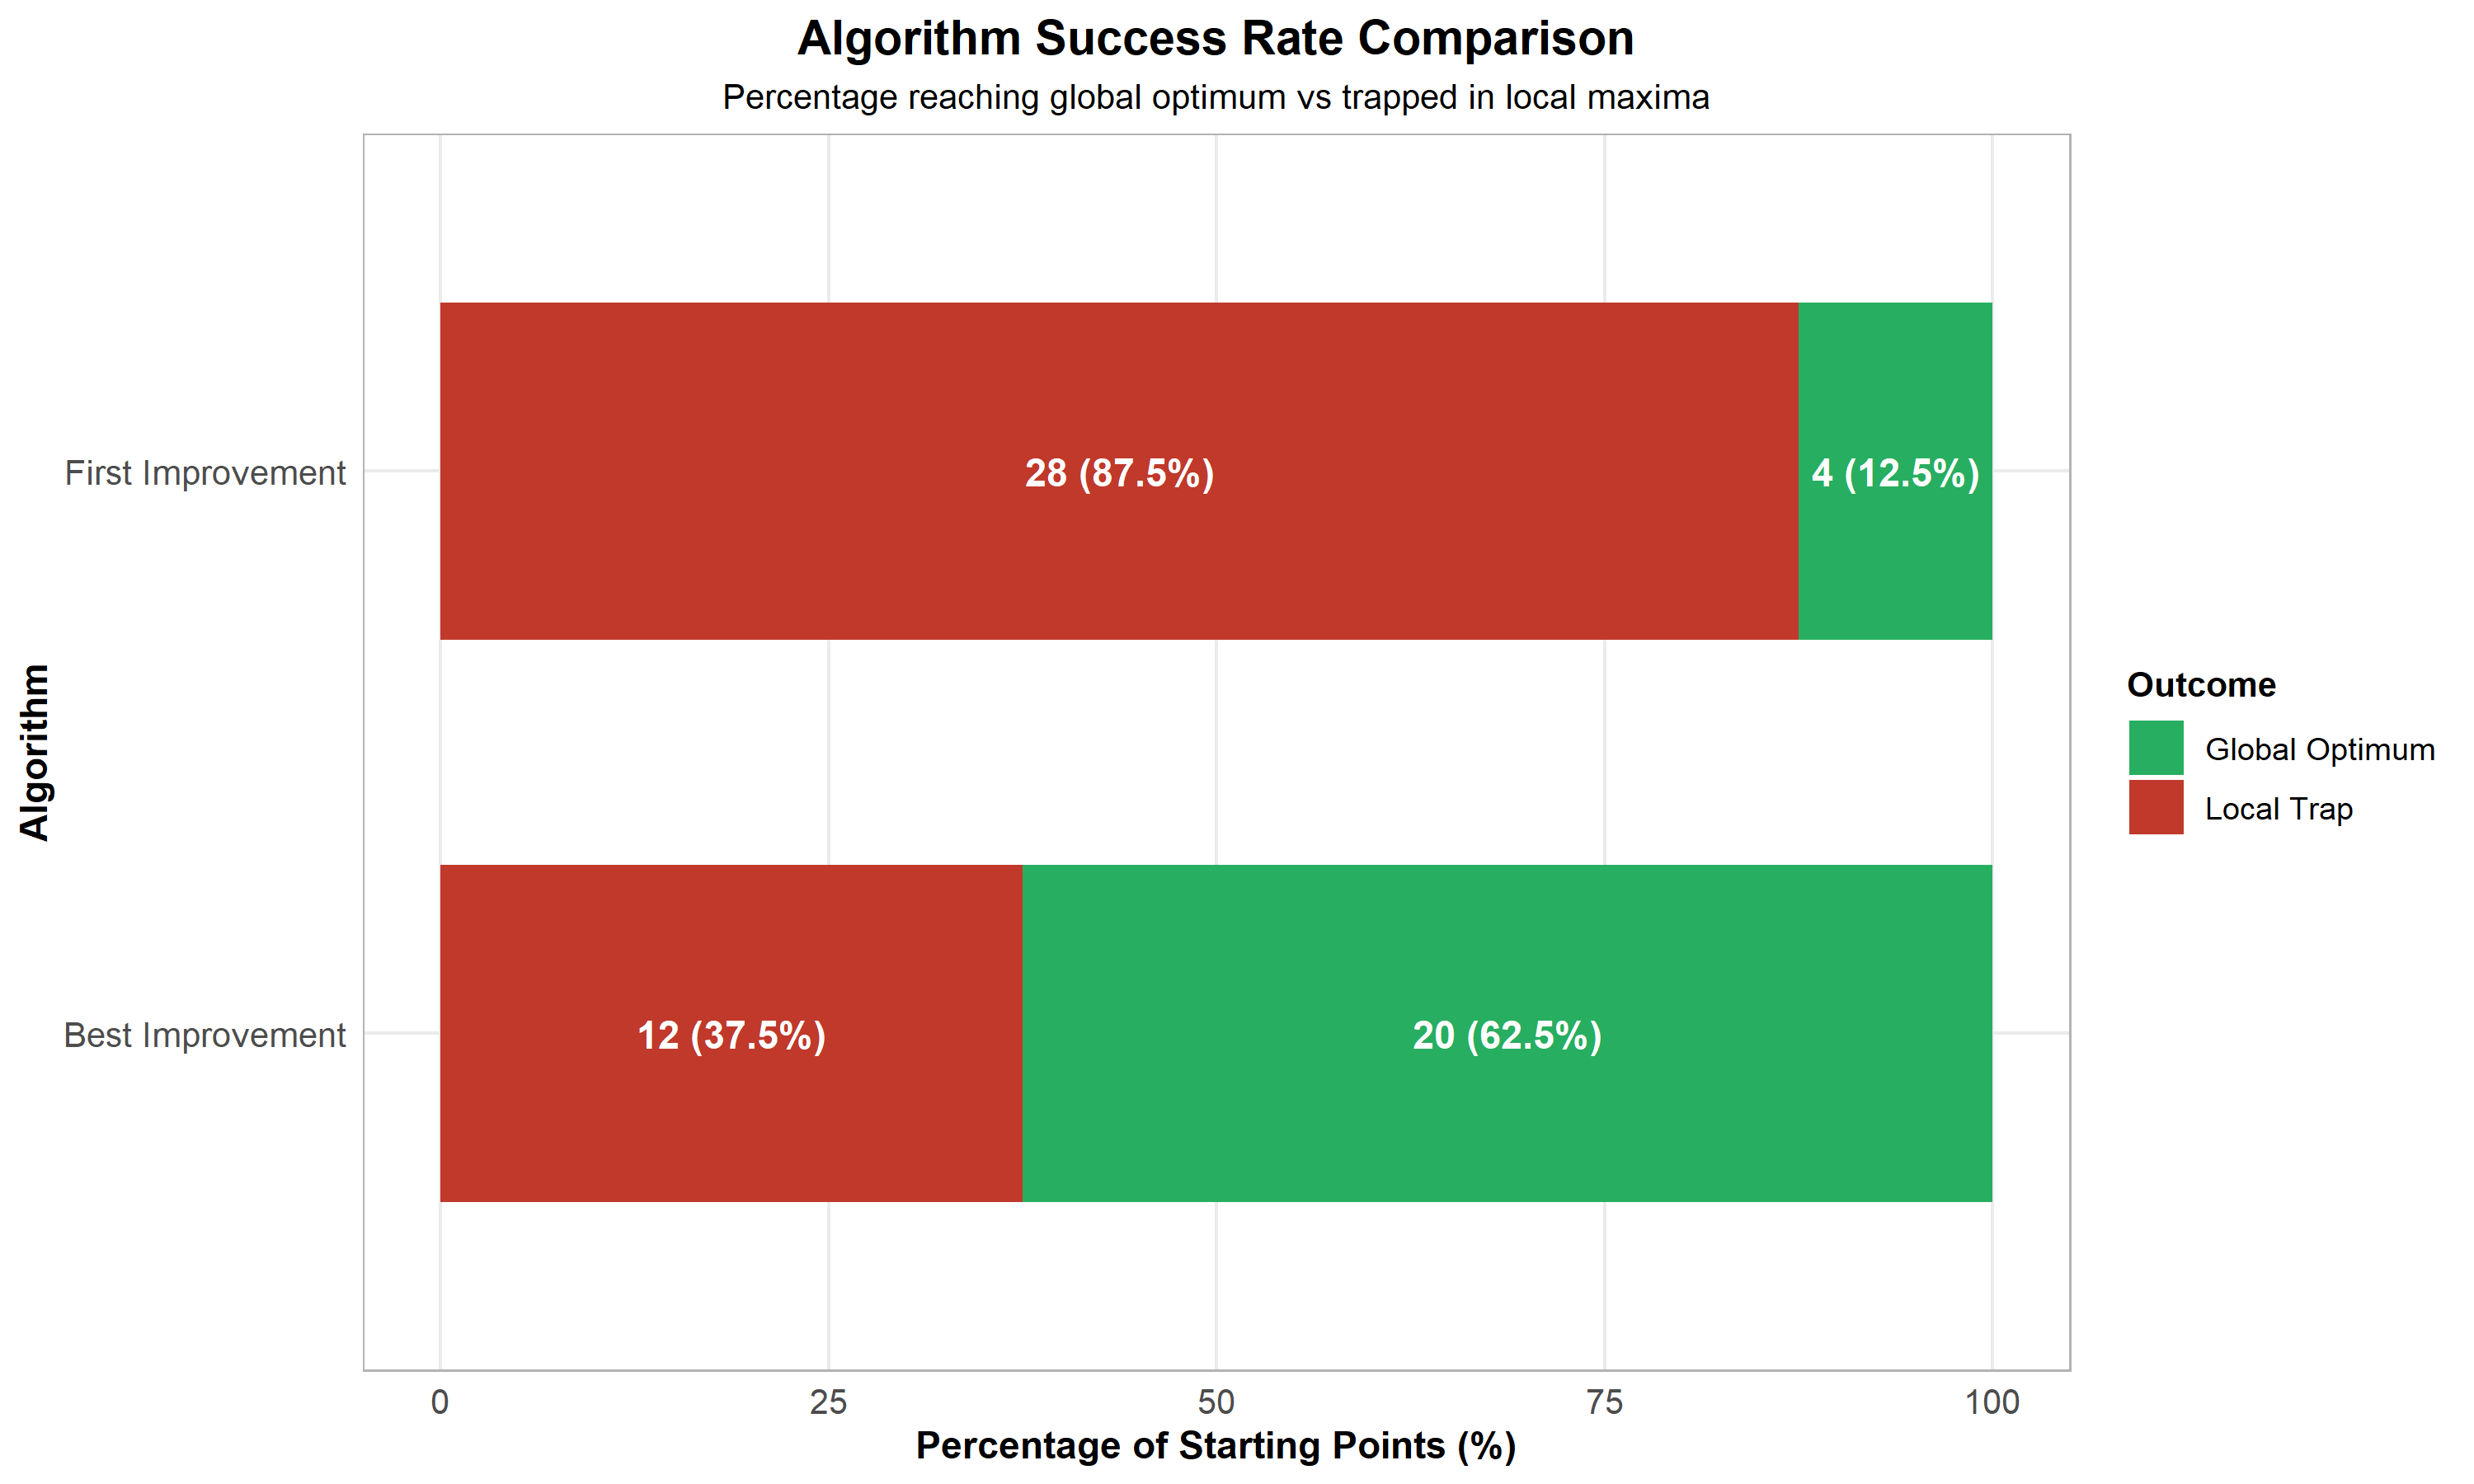
\includegraphics[width=5.5in]{../success_rate.png}
\par\textit{Figure 4: Success rates showing percentage reaching global optimum vs trapped in local maxima}
\end{center}

\begin{center}
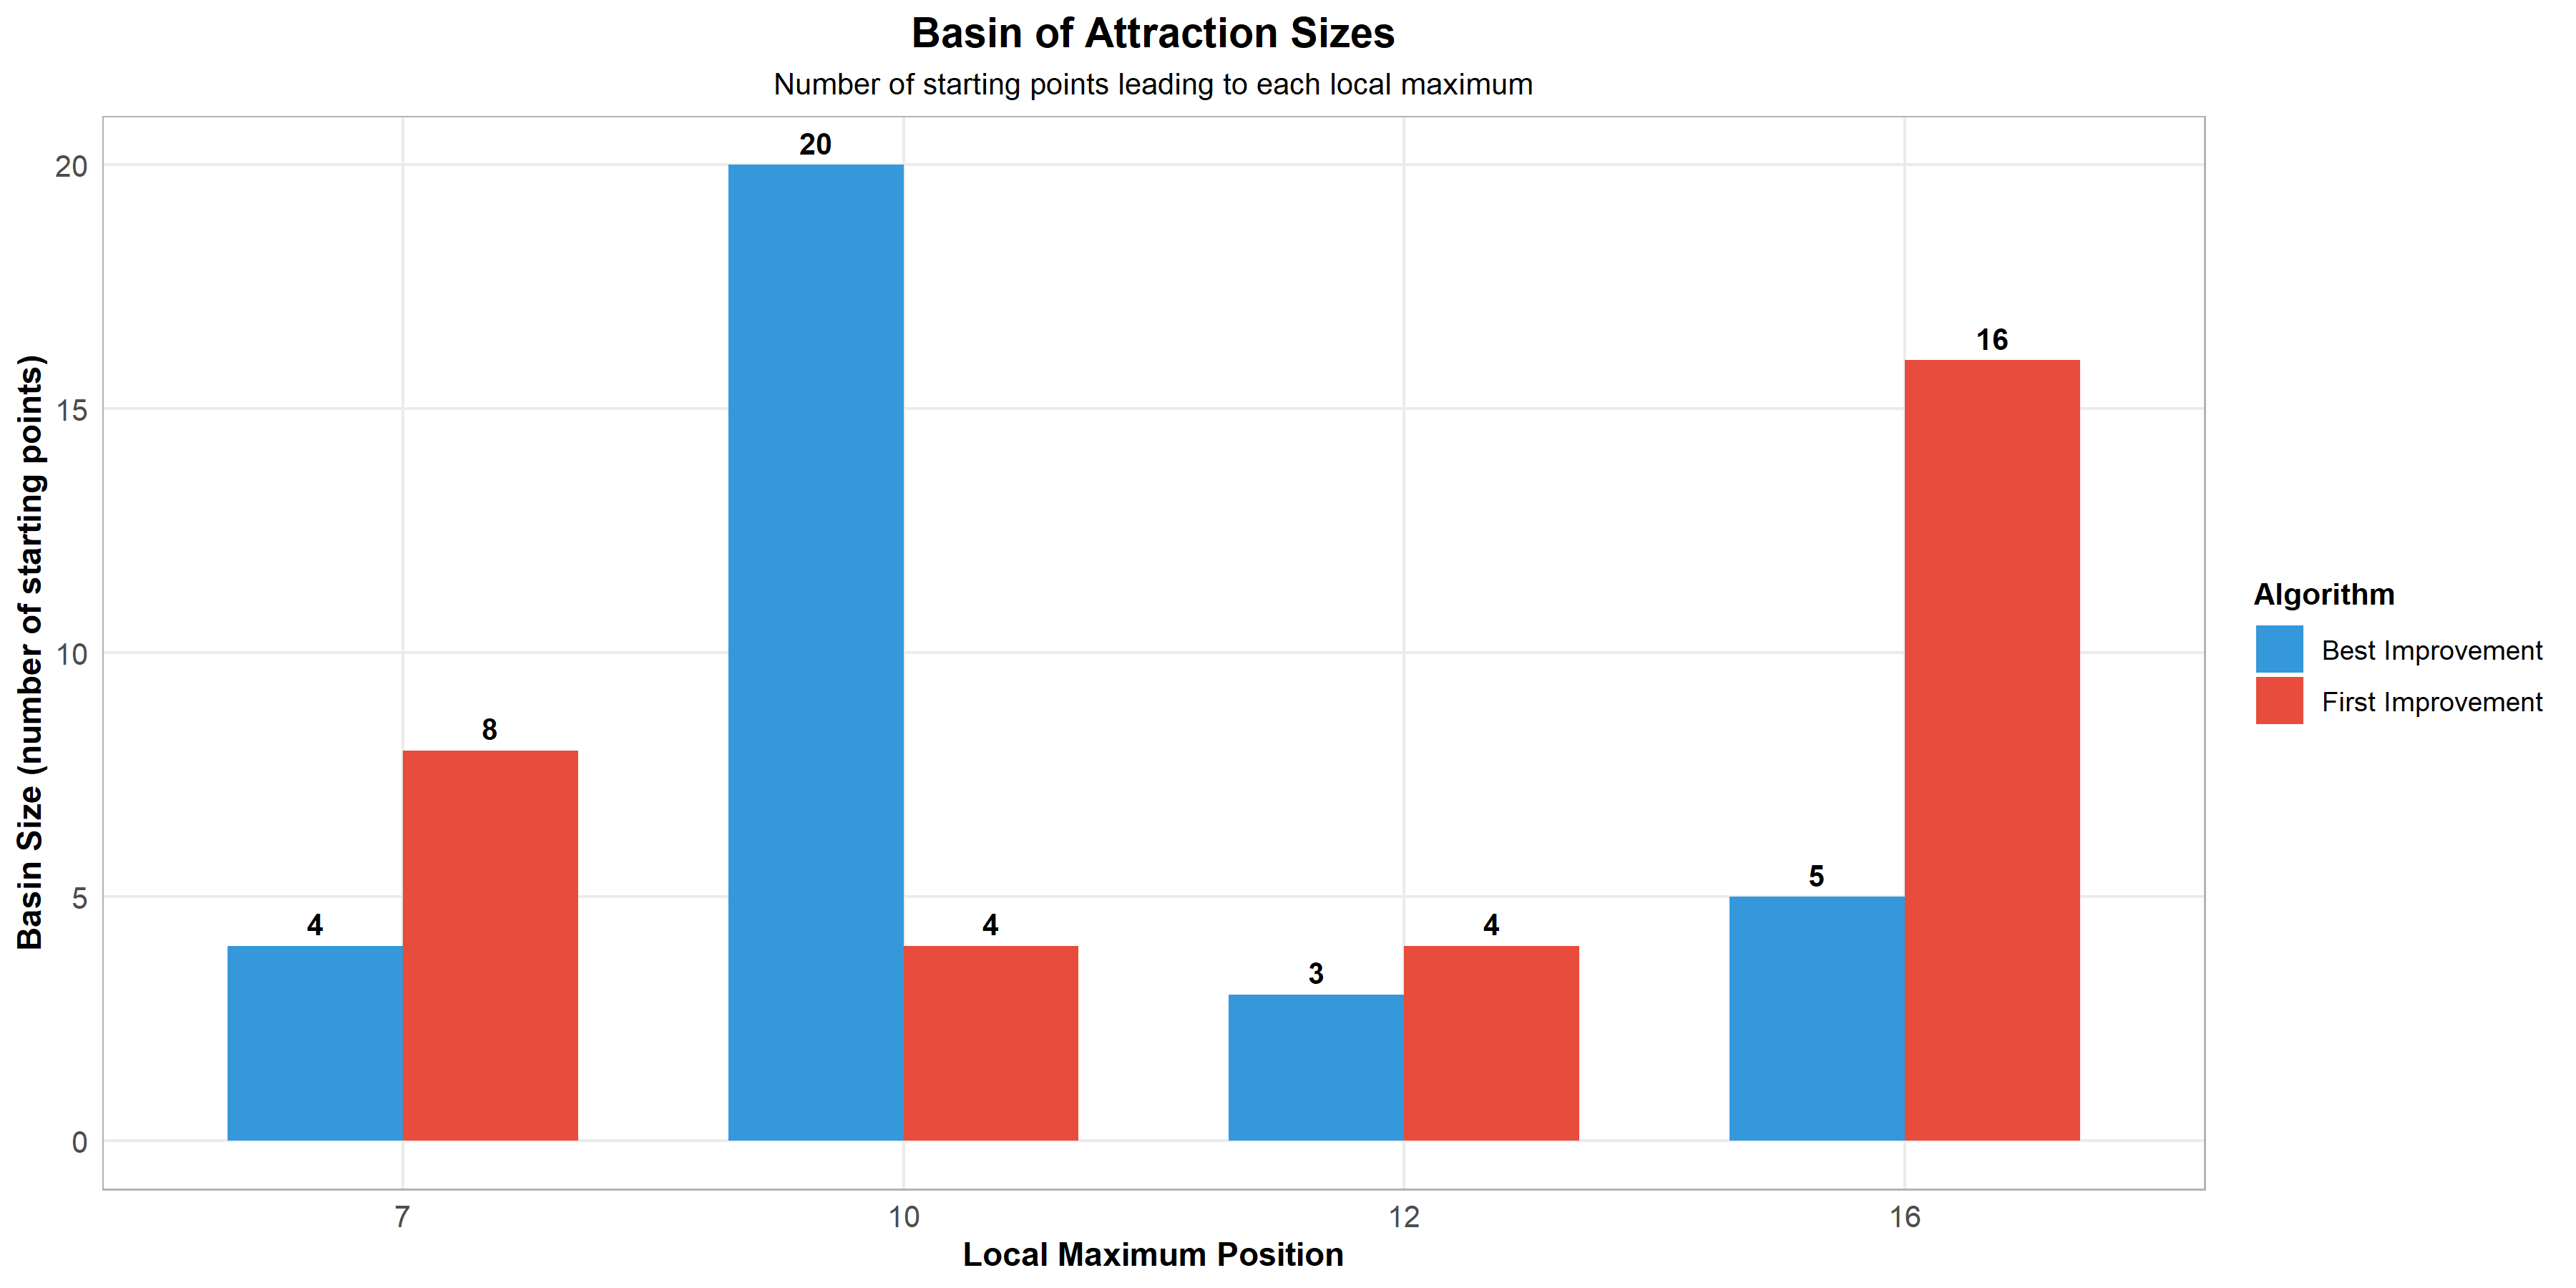
\includegraphics[width=5.5in]{../basin_comparison.png}
\par\textit{Figure 5: Basin of attraction sizes for each local maximum}
\end{center}

With multiple restarts, First Improvement can approach Best
Improvement\textquotesingle s reliability, but requires three to five
runs to achieve comparable success rates, consuming the same or more
total evaluations.

\textbf{Parameter Influence}

The selection strategy profoundly
impacts performance. Changing from First to Best Improvement doubles
global convergence rate. We attempted optimizing First Improvement
through different neighbor evaluation orders and randomization, but
improvements were marginal. Switching to Best Improvement provided the
only substantial performance gain.

\begin{center}
\textbf{CONCLUSIONS}
\end{center}

\textbf{Key Findings}

This study demonstrates that fitness landscape difficulty
is not intrinsic but emerges from algorithm-landscape interaction. The
same objective function appears dramatically different to Best
Improvement versus First Improvement. Strategy dominates structure: how
you search matters as much as what you search. Best
Improvement\textquotesingle s exhaustive evaluation provides robustness.
By surveying all neighbors before moving, it chooses steepest ascent and
avoids most traps. First Improvement\textquotesingle s myopic decisions
create path dependence. Accepting the first improvement without checking
alternatives introduces directional bias that fragments the search
space. The computational trade-off favors Best Improvement: spending
eighty percent more computation per iteration yields one hundred percent
more successful outcomes. This represents excellent return on investment
for most practical applications.

\textbf{Practical Implications}

When
computational budget allows, prefer Best Improvement for superior
robustness. Accept the modest cost increase as worthwhile investment.
When speed is critical, First Improvement offers faster iterations but
requires multiple restarts to achieve acceptable reliability. For
unknown landscapes, start with Best Improvement to assess difficulty
before considering faster but less reliable alternatives.

\textbf{Future Research}

Two promising directions emerge. First, investigate adaptive
hybrid strategies that dynamically switch between Best and First
Improvement based on neighborhood characteristics. When neighbors show
high fitness variance, use Best Improvement for high-stakes decisions.
When variance is low, use First Improvement to save cost. This could
combine robustness with efficiency. Second, quantify how randomizing
neighbor evaluation order affects First Improvement\textquotesingle s
basin fragmentation. While our preliminary tests show modest
improvement, systematic study could reveal whether randomization truly
eliminates directional bias or merely redistributes it.

\begin{center}
\textbf{BIBLIOGRAPHY}
\end{center}

Russell, S., \& Norvig, P. (2020). Artificial Intelligence: A Modern
Approach (4th edition).

Pearson Education. Chapter 4 covers local search algorithms including
Hill Climbing variants. Talbi, E.-G. (2009).

Metaheuristics: From Design to Implementation. John Wiley \& Sons.
Chapter 3 provides detailed analysis of Hill Climbing strategies.

University course materials on Introduction to Artificial Intelligence,
including lecture notes on optimization algorithms and fitness landscape
analysis.

Wikipedia articles on Hill Climbing and Fitness Landscapes provided
background information and historical context.

Wolfram Alpha was used for verifying analytical properties of the cubic
function and calculating critical points.

Various educational YouTube channels provided supplementary visual
explanations of fitness landscapes and algorithm trajectories.

\end{document}
